\chapter{Konzept}
Die ursprüngliche Idee zur Implementation eines GA-HMM Frameworks war es bereits existierende Python Libraries für HMMs und Genetische Algorithmen zu kombinieren. Da ich jedoch keine Libraries gefunden habe, welche meinen hohen Ansprüchen an Erweiterbarkeit genügten habe ich den Code von Grund auf konstruiert. Meine Erfahrung, des aus dieser Entscheidung resultierenden Schaffensprozesses, lässt sich adäquat durch folgendes Zitat beschreiben.
"The basic idea behind the from scratch-oriented approach is the apparent simplicity of metaheuristic code. Programmers are tempted to develop themselves their codes. Therefore, they are faced with several problems: the development requires time and energy, and it is error prone and difficult to maintain and evolve" \cite*{MetaheuristicsEGT}
Im folgenden werde die Funktionsweise des Frameworks beschreiben und darauf eingehen was bei einer Kombination von Hidden Markov Modellen mit einem genetischen Algorithmus zu beachten ist.

\subsection*{Die Fitness Funktion}
Unser Ziel ist Parameter $\lambda = \pi, B, A$ zu finden welche die Wahrscheinlichkeit einer Menge an Observationssequenzen maximieren. Die Fitness Funktion eines Chromosoms ist daher die durchschnittliche Log-Wahrscheinlichkeit der Observationssequenzen für den Phänotyp des Chromosoms.
\begin{equation*}
    fitness(\lambda) = \frac{\sum_{\text{alle O}} log[P(O \mid \lambda)] }{\text{anzahl O}} 
\end{equation*}


\subsection*{Genetische Operatoren}
Die Genetischen Operatoren welche implementiert wurden sind

\subsubsection*{Crossover Operatoren}


\subsubsection*{Mutations Operatoren}
Um zu garantieren, dass die Struktur eines Hidden Markov Models nicht verändert wird gibt es verschiedene Kategorien.
- Nur Emissionsmatrix mutieren
- Maske erstellen und nur maskierte Werte Mutieren
- Werte die Nicht verändert werden dürfen nicht in die Chromosom-Representation aufnehmen.

\subsection*{Ablauf des GA-HMM}
Der GA-HMM erweitert den Ablauf eines klassischen genetischen Algorithmus um einige Schritte. Durch den Reproduktionsschritt können Chromosome erzeugt werden, welche unzulässige HMM-Parameter representieren. Zum Beispiel kann durch eine Mutation oder ein Crossover die Reihenstochastizität verletzt werden. Um solche unzulässigen Repräsentationen in den folgenden Schritten zu verhindern folgt nach dem Reproduktionsschritt ein \textbf{Normalisierungs-Schritt}. Solch eine Transformation unzulässiger Lösung in zulässige Lösungen ist bekannt als \textbf{Reparatur Strategie} \cite*{MetaheuristicsEGT}. Des weiteren findet vor der Normalisierung ein optionaler \textbf{Smoothing-Schritt} statt um Overfitting entgegenzuwirken. Der Baum-Welch Algorithmus kann vor dem genetischen Algorithmus, danach und zwischendurch angewendet werden. Dadurch sind Relay-Hybridisierung, Teamwork-Hybridisierung und auch keine Hybridisierung innerhalb eines Frameworks durch Parameter für die einzelnen Baum-Welch Schritte realisierbar.

\begin{figure}[h!]
    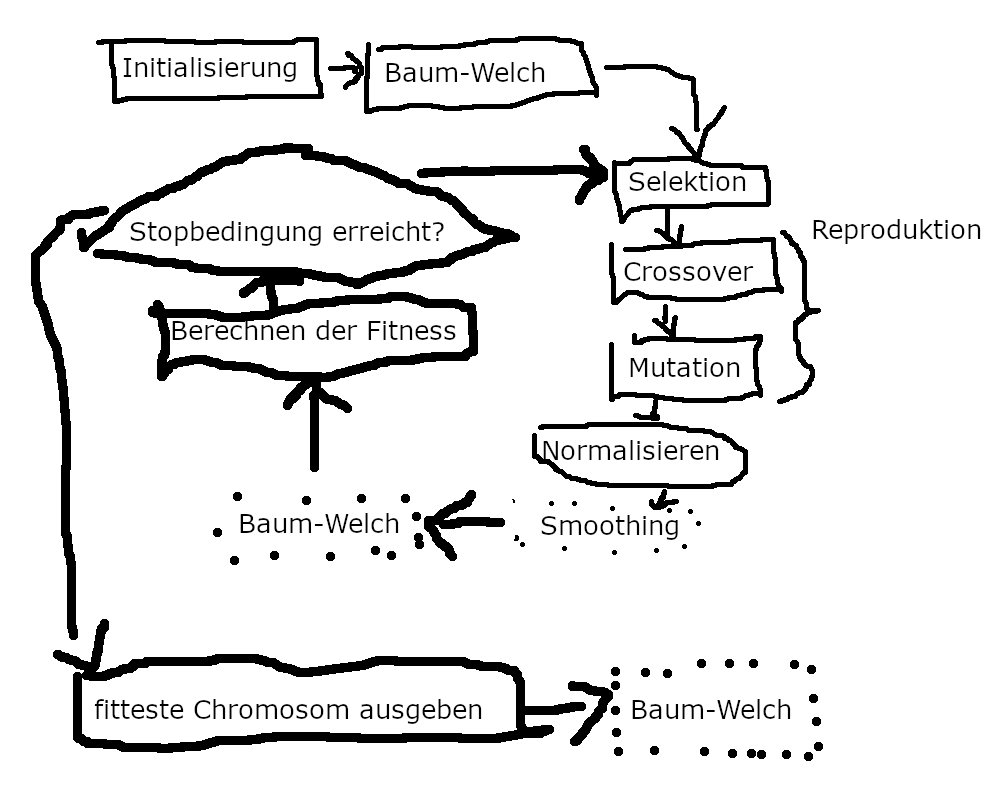
\includegraphics[scale=1.0]{images/GA-HMM_Flowchart.png}
    \caption{Ablauf des GA-HMM}
    \label{fig:gahmm_flowchart}
\end{figure}

